\section{引言}
\label{sec:intro}

投稿准备通常横跨实验代码、数据、图表与论文源码多个目录。dsh-leaf 将整个目录视为一个
LaTeX 项目：普通对话负责实验与绘图，写作视图负责源码、编译与 PDF 审阅。

本文的主要观察是：把编译入口固定为主文档，并让章节文件共享同一个写作视图，可以显著减少
在多个工具之间搬运上下文的时间。示意结果见图~\ref{fig:workflow}。

\begin{figure}[htbp]
  \centering
  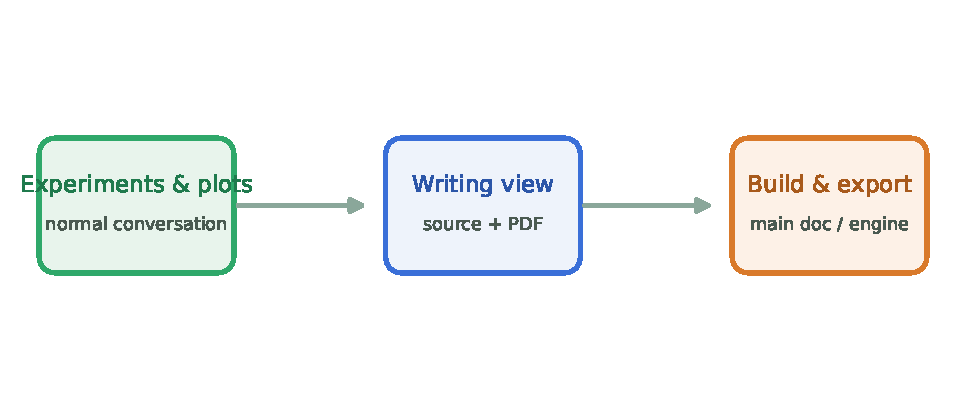
\includegraphics[width=0.72\linewidth]{figures/workflow.pdf}
  \caption{dsh-leaf 的工作流程示意：资料整理、绘图、写作、编译与导出共享同一个工作区。}
  \label{fig:workflow}
\end{figure}

相关工作可参考~\cite{lamport1994latex}。
